% %% file: template.tex = LaTeX template for article-like report 
%% init: sometime 1993
%% last: Feb  8 2015  Rob Rutten  Deil
%% site: http://www.staff.science.uu.nl/~rutte101/rrweb/rjr-edu/manuals/student-report/

%% First read ``latex-bibtex-simple-manual.txt'' at
%% http://www.staff.science.uu.nl/~rutte101/Report_recipe.html

%% Start your report production by copying this file into your XXXX.tex.
%% Small changes to the header part will make it an A&A or ApJ manuscript.

%%%%%%%%%%%%%%%%%%%%%%%%%%%%%%%%%%%%%%%%%%%%%%%%%%%%%%%%%%%%%%%%%%%%%%%%%%%%
%\documentclass{aa}   %% Astronomy & Astrophysics style class
\documentclass[a4paper]{report}
\usepackage{geometry}
\geometry{a4paper}
\usepackage{graphicx,url,twoopt}
\usepackage{subcaption}
\usepackage{enumitem}
\usepackage{amsmath}
\usepackage[varg]{txfonts}           %% A&A font choice
%\usepackage{hyperref}                %% for pdflatex
%%\usepackage[breaklinks]{hyperref}  %% for latex+dvips
%%\usepackage{breakurl}              %% for latex+dvips
%\usepackage{pdfcomment}              %% for popup acronym meanings
%\usepackage{acronym}                 %% for popup acronym meanings
\usepackage{calrsfs}
\DeclareMathAlphabet{\pazocal}{OMS}{zplm}{m}{n}

\usepackage{natbib}
% \hypersetup{
%   colorlinks=true,   %% links colored instead of frames
%   urlcolor=blue,     %% external hyperlinks
%   linkcolor=red,     %% internal latex links (eg Fig)
% }

 %\bibpunct{(}{)}{;}{a}{}{,}    %% natbib cite format used by A&A and ApJ
 
%\pagestyle{plain}   %% undo the fancy A&A pagestyle 


%%%%%%%%%%%%%%%%%%%%%%%%%%%%%%%%%%%%%%%%%%%%%%%%%%%%%%%%%%%%%%%%%%%%%%%%%%%%
\begin{document}  

%\twocolumn[{%
\vspace*{4ex}

\begin{center}
  {\Large \bf blablabla}\\[4ex]
  {\large \bf Andreas Ellewsen$^1$}\\[4ex]
  \begin{minipage}[t]{15cm}
        $^1$ Institute of Theoretical Astrophysics, University of Oslo, P.O. Box 1029 Blindern, N-0315 Oslo, Norway\\
             
        
    {\bf Abstract.} I compute the density perturbations, and velocities of dark matter and baryons. As well as the gravitational potentials $\Phi$ and $\Psi$. More importantly I also find $\Theta_0$.
    
  \vspace*{2ex}
  \end{minipage}
\end{center}
%}]
%\onecolumn
%%%%%%%%%%%%%%%%%%%%%%%%%%%%%%%%%%%%%%%%%%%%%%%%%%%%%%%%%%%%%%%%%%%%%%%%%%%%
\section{Introduction}\label{sec:introduction}
%%%%%%%%%%%%%%%%%%%%%%%%%%%%%%%%%%%%%%%%%%%%%%%%%%%%%%%%%%%%%%%%%%%%%%%%%%%%
In this project I will follow the algorithm presented in Callin (2005)[1] for simulating the cosmic microwave background.  
This is part three of four for this project.

In the first part I set up the background cosmology of the universe, and made a function that could find the conformal time as a function of $x$. In the second part I computed the electron fraction, electron density, optical depth and visibility function for times around and during recombination. 

In this part I will use some of these functions along with the Einstein-Boltzmann equations without polarization and neutrinos to compute the density perturbations, and velocities of dark matter and baryons. As well as the temperature multipoles $\Theta_l$.

As prevously done I will continue building on the skeleton code provided.

%%%%%%%%%%%%%%%%%%%%%%%%%%%%%%%%%%%%%%%%%%%%%%%%%%%%%%%%%%%%%%%%%%%%%%%%%%%%
\section{Equations}\label{sec:Equations}
%%%%%%%%%%%%%%%%%%%%%%%%%%%%%%%%%%%%%%%%%%%%%%%%%%%%%%%%%%%%%%%%%%%%%%%%%%%%
The full set of Einstein-Boltzmann equations without polarization and neutrinos read
\begin{align}
 \Theta^\prime_0 =& -\frac{ck}{\pazocal{H}}\Theta_1 - \Phi^\prime\\
 \Theta^\prime_1 =& \frac{ck}{3\pazocal{H}}\Theta_0 - \frac{2ck}{3\pazocal{H}}\Psi + \tau^\prime\bigg[\Theta_1+\frac{1}{3}v_b\bigg]\\
 \Theta_l^\prime =& \frac{lck}{(2l+1)\pazocal{H}}\Theta_{l-1} - \frac{(l+1)ck}{(2l+1)\pazocal{H}}\Theta_{l+1} + \tau^\prime\bigg[\Theta_l-\frac{1}{10}\Theta_l\delta_{l,2} \bigg], 2\le l < l_{max}\\
 \Theta_l^\prime =& \frac{ck}{\pazocal{H}}\Theta_{l-1} - c\frac{l+1}{\pazocal{H}\eta(x)}\Theta_l + \tau^\prime\Theta_l, l=l_{max}\\
 \delta^\prime =&\frac{ck}{\pazocal{H}}v -3\Phi^\prime\\
 v^\prime =& -v -\frac{ck}{\pazocal{H}}\Psi\\
 \delta^\prime_b =& \frac{ck}{\pazocal{H}}v_b - 3\Phi^\prime\\
 v_b^\prime =& -v_b - \frac{ck}{\pazocal{H}}\Psi +\tau^\prime R(3\Theta_1+v_b)\\
 \Phi^\prime =& \Psi - \frac{c^2 k^2}{3\pazocal{H}^2}\Phi + \frac{H_0^2}{2\pazocal{H}^2}\bigg[\Omega_m a^{-1}\delta + \Omega_b a^{-1}\delta_b +4\Omega_r a^{-2}\Theta_0 \bigg]\\
 R =& \frac{4\Omega_r}{3\Omega_b a}.
\end{align}

These equations are the ones we will use when we are not in the tight coupling regime. When in the tight coupling regime the factor $(3\Theta_1+v_b)$ is very close to zero. In the equation for $v_b^\prime$ this is multiplied by $\tau^\prime$ which is very large in, making this equation terribly unstable. The same thing makes the equation for $\Theta^\prime_1$ unstable. Because of this one expand $(3\Theta_1+v_b)$ in powers of $1/tau^\prime$. This results in 
a slight change in the set of equations for $v_b^\prime$ and $\Theta_l$.

\begin{align} 
q &= \frac{-[(1-2R)\tau^\prime + (1+R)\tau^{\prime\prime}](3\Theta_1+v_b) - \frac{ck}{\pazocal{H}}\Psi + (1-\frac{\pazocal{H}^\prime}{\pazocal{H}})\frac{ck}{\pazocal{H}}(-\Theta_0+2\Theta_2) - \frac{ck}{\pazocal{H}}\Theta_0^\prime} {(1+R)\tau^\prime + \frac{\pazocal{H}^\prime}{\pazocal{H}} - 1}\\
v_b^\prime &= \frac{1}{1+R}\bigg[ -v_b - \frac{ck}{\pazocal{H}}\Psi + R(q + \frac{ck}{\pazocal{H}}(-\Theta_0+2\Theta_2)-\frac{ck}{\pazocal{H}}\Psi) \bigg]\\
\Theta_1^\prime &= \frac{1}{3}(q - v_b^\prime).
 \end{align}

So far I have not stated what tight coupling means. Basically because of the mathematical operations we have done, like expanding in powers of $1/tau^\prime$, we end up with some conditions on when these equations above can be used. The conditions are $|ck/(\pazocal{H}\tau^\prime)| < 1/10$, $|\tau^\prime|>10$, and that the time is before recombination.
 

%%%%%%%%%%%%%%%%%%%%%%%%%%%%%%%%%%%%%%%%%%%%%%%%%%%%%%%%%%%%%%%%%%%%%%%%%%%%
\section{Implementation}\label{sec:Imp}
%%%%%%%%%%%%%%%%%%%%%%%%%%%%%%%%%%%%%%%%%%%%%%%%%%%%%%%%%%%%%%%%%%%%%%%%%%%%
The way to solve all these equations is to first make a function that finds the time where tight coupling ends.
Note that this function clearly depends on which k mode we are working on.

For each k we insert the initial conditions, and then run through every value of x from some start value early in the universe. In this case I have chosen to use the $x$ value corresponding to $a_{init} = 10^{-8}$.
At some point through this the x value becomes larger than the x value indicating the end of tight coupling. There we change the equations for the relevant quantities, and continue on until we reach today.
This has to be done for all k values. I have chosen to set the limit at $k=100$ so far. With this low k value the program completes in less than five minutes.

It should also be said that we limit our number of $l$'s to six. This can be done because we are using line of sight integration. Historically people used to include thousands of variables to trace multipoles. If we had to use this the program would use days or weeks instead of minutes.

%%%%%%%%%%%%%%%%%%%%%%%%%%%%%%%%%%%%%%%%%%%%%%%%%%%%%%%%%%%%%%%%%%%%%%%%%%%%
\section{Results}\label{sec:results}
%%%%%%%%%%%%%%%%%%%%%%%%%%%%%%%%%%%%%%%%%%%%%%%%%%%%%%%%%%%%%%%%%%%%%%%%%%%%
To get a good distribution of k modes we use a quadratic distribution in k such that
\begin{equation}
 k_i = k_{max} +(k_{max}-k_{min})(i/100)^2,
\end{equation}
where $k_{max} = 1000H_0/c$, and $k_{min} = 0.1H_0/c$.

The results show the various quantities for six differnent k values. These k values are $k_1,k_5,k_{10},k_{40},k_{60},k_{100}$. 

\begin{figure}
\begin{subfigure}{.5\textwidth}
  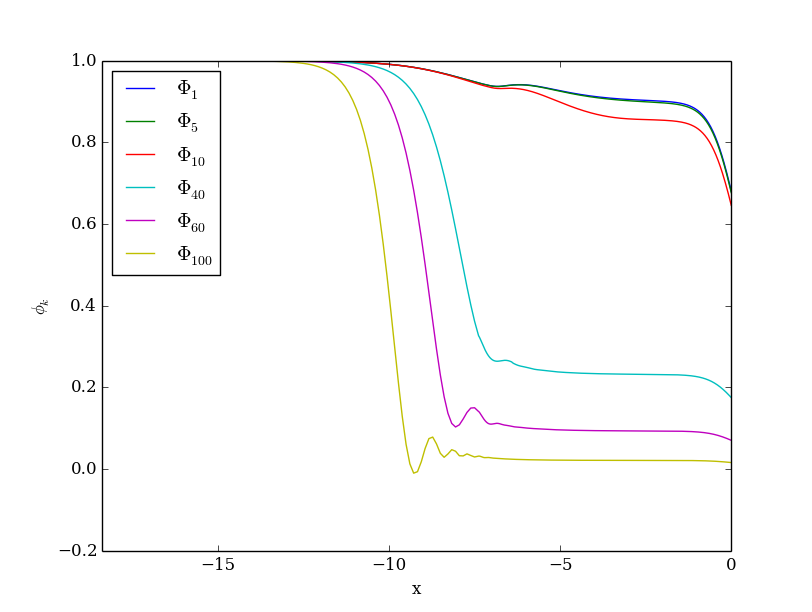
\includegraphics[width=\textwidth]{Phi.png}
 \caption{The plot for $\Phi$ for six different k's.}
 \label{fig:Phi}
\end{subfigure}
\begin{subfigure}{.5\textwidth}
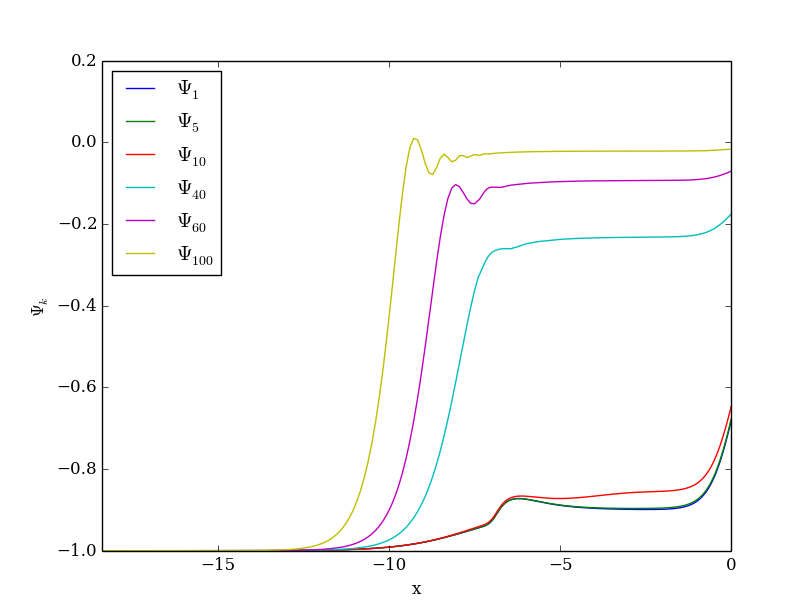
\includegraphics[width=\textwidth]{Psi.png}
 \caption{The plot for $\Psi$ for six different k's.}
 \label{fig:Psi}
\end{subfigure}
\caption{We note that the plots seem to be the inverse of each other.}
\end{figure}

\begin{figure}
\begin{subfigure}{.5\textwidth}
  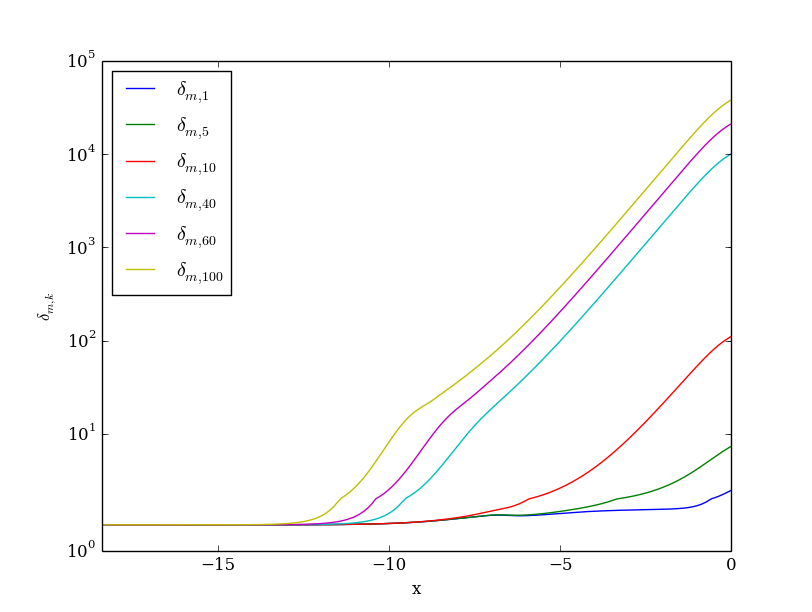
\includegraphics[width=\textwidth]{delta.png}
 \caption{The plot for $\delta$ for six different k's.}
 \label{fig:delta}
\end{subfigure}
\begin{subfigure}{.5\textwidth}
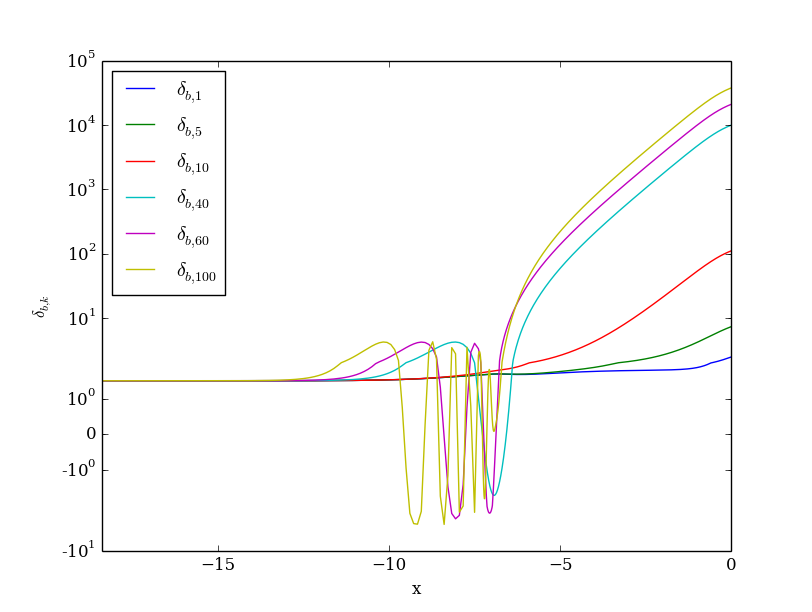
\includegraphics[width=\textwidth]{deltab.png}
 \caption{The plot for $\delta_b$ for six different k's.}
 \label{fig:deltab}
\end{subfigure}
\caption{Note the special y axis on the plot for $\delta_b$. The dark matter perturbations behave nicely. The higher the mode the earlier it can start growing, just as expected due to the fact that forces don't propagate instantaneously. Note also that all the dark matter perturbations remain positive. This is not the case for baryons. When we start approaching recombination all the higher order modes start oscillating, and it is only after recombination is done that they are allowed to start growing again, and now the can behave like dark matter.}
\end{figure}

\begin{figure}
\begin{subfigure}{.5\textwidth}
  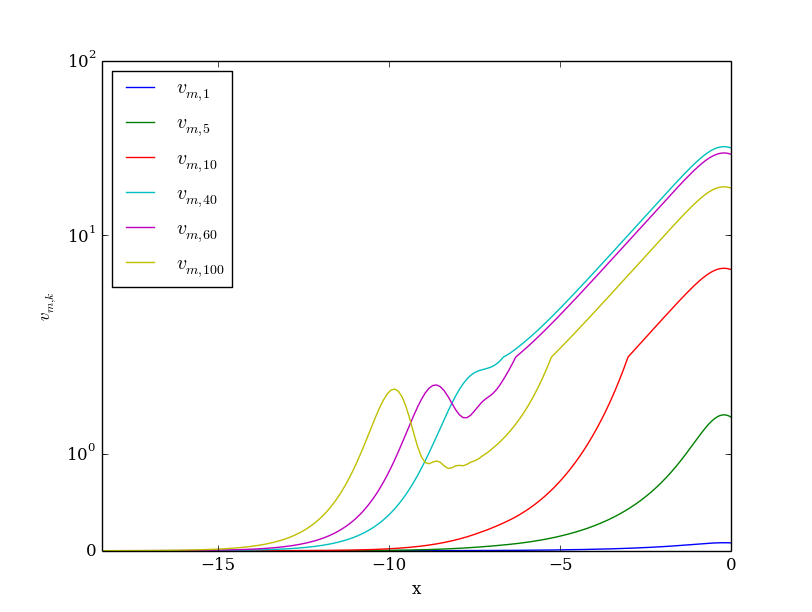
\includegraphics[width=\textwidth]{v.png}
 \caption{The plot for $v$ for six different k's.}
 \label{fig:v}
\end{subfigure}
\begin{subfigure}{.5\textwidth}
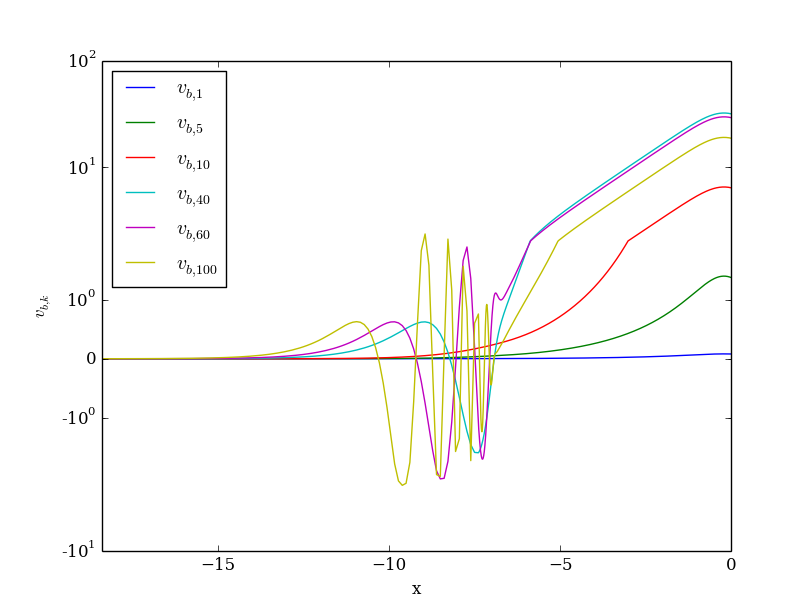
\includegraphics[width=\textwidth]{vb.png}
 \caption{The plot for $v_b$ for six different k's.}
 \label{fig:vb}
\end{subfigure}
\caption{}
\end{figure}

\begin{figure}
 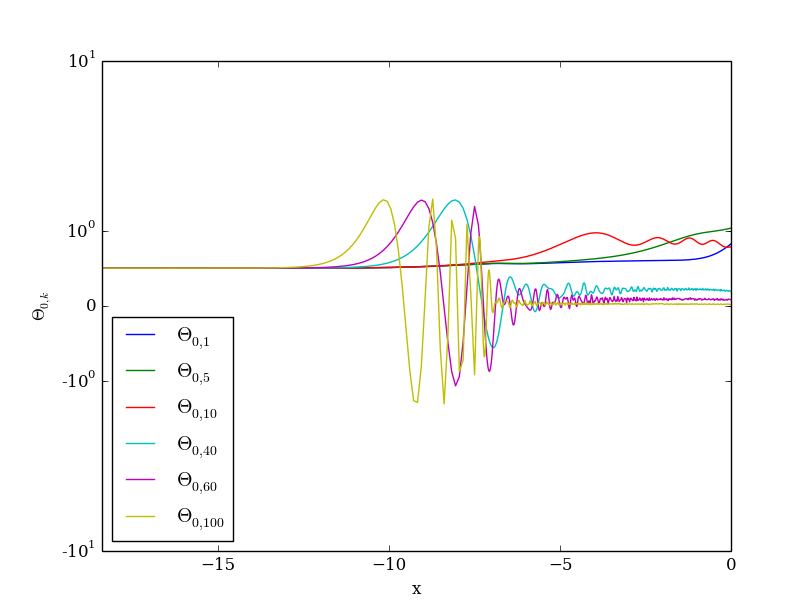
\includegraphics[width=\textwidth]{Theta0.png}
 \caption{The plot for $\Theta_0$ for six different k's.}
 \label{fig:Phi}
\end{figure}





%%%%%%%%%%%%%%%%%%%%%%%%%%%%%%%%%%%%%%%%%%%%%%%%%%%%%%%%%%%%%%%%%%%%%%%%%%%%
\section{Conclusions} \label{sec:conclusions}
%%%%%%%%%%%%%%%%%%%%%%%%%%%%%%%%%%%%%%%%%%%%%%%%%%%%%%%%%%%%%%%%%%%%%%%%%%%%

%%%%%%%%%%%%%%%%%%%%%%%%%%%%%%%%%%%%%%%%%%%%%%%%%%%%%%%%%%%%%%%%%%%%%%%%%%%%
\section{References}
%%%%%%%%%%%%%%%%%%%%%%%%%%%%%%%%%%%%%%%%%%%%%%%%%%%%%%%%%%%%%%%%%%%%%%%%%%%%
\begin{enumerate}[label= {[}\arabic*{]} ]
 \item P. Callin, astro-ph/0606683
\end{enumerate}



%\bibliographystyle{aa-note} %% aa.bst but adding links and notes to references
%\raggedright              %% only for adsaa with dvips, not for pdflatex
%\bibliographystyle{unsrt}
%\bibliography{bibliography}{}       %% XXX.bib = your Bibtex entries copied from ADS

\onecolumn 
%%%%%%%%%%%%%%%%%%%%%%%%%%%%%%%%%%%%%%%%%%%%%%%%%%%%%%%%%%%%%%%%%%%%%%%%%%%%
\section{Source code}\label{sec:files}
%%%%%%%%%%%%%%%%%%%%%%%%%%%%%%%%%%%%%%%%%%%%%%%%%%%%%%%%%%%%%%%%%%%%%%%%%%%%
The source code for the evolution\_mod file is included for inspection. Note that the code makes use of several different files, one with various parameters, as well as the ODE solver, and the spline. This includes all files used in previous parts of the project as well.



%%%%%%%%%%%%%%%%%%%%%%%%%%%%%%%%%%%%%%%%%%%%%%%%%%%%%%%%%%%%%%%%%%%%%%%%%%%%
%\begin{acknowledgements}
%\end{acknowledgements}

\end{document}